\documentclass{article}

% if you need to pass options to natbib, use, e.g.:
%     \PassOptionsToPackage{numbers, compress}{natbib}
% before loading neurips_2020

% ready for submission
% \usepackage{neurips_2020}

% to compile a preprint version, e.g., for submission to arXiv, add add the
% [preprint] option:
    \usepackage[preprint]{neurips_2020}

% to compile a camera-ready version, add the [final] option, e.g.:
%     \usepackage[final]{neurips_2020}

% to avoid loading the natbib package, add option nonatbib:
     % \usepackage[natbib]{neurips_2020}

\usepackage[utf8]{inputenc} % allow utf-8 input
\usepackage[T1]{fontenc}    % use 8-bit T1 fonts
\usepackage{hyperref}       % hyperlinks
\usepackage{url}            % simple URL typesetting
\usepackage{booktabs}       % professional-quality tables
\usepackage{amsfonts}       % blackboard math symbols
\usepackage{nicefrac}       % compact symbols for 1/2, etc.
\usepackage{microtype}      % microtypography
\usepackage{algorithm}
\usepackage{algorithmic}
\usepackage{mathtools}
\usepackage{graphicx}  % allows inclusion of PDF, PNG and JPG images


\newlength\myindent
\setlength\myindent{2em}
\newcommand\bindent{%
  \begingroup
  \setlength{\itemindent}{\myindent}
  \addtolength{\algorithmicindent}{\myindent}
}
\newcommand\eindent{\endgroup}


\bibliographystyle{unsrt}

\title{FedExP in Flower}

% The \author macro works with any number of authors. There are two commands
% used to separate the names and addresses of multiple authors: \And and \AND.
%
% Using \And between authors leaves it to LaTeX to determine where to break the
% lines. Using \AND forces a line break at that point. So, if LaTeX puts 3 of 4
% authors names on the first line, and the last on the second line, try using
% \AND instead of \And before the third author name.

\author{%
  Henry Batchelor\\
  \texttt{htb27@cam.ac.uk} \\
  % examples of more authors
  % \And
  % Coauthor \\
  % Affiliation \\
  % Address \\
  % \texttt{email} \\
  % \AND
  % Coauthor \\
  % Affiliation \\
  % Address \\
  % \texttt{email} \\
  % \And
  % Coauthor \\
  % Affiliation \\
  % Address \\
  % \texttt{email} \\
  % \And
  % Coauthor \\
  % Affiliation \\
  % Address \\
  % \texttt{email} \\
}

\begin{document}

\maketitle

\begin{abstract}
  The goal of this project is to implement the FedExP algorithm \cite{FedExP}, which aims to improve the performance over FedAvg by dynamically altering the server step size, inside of Flower \cite{flower} a framework for Federated Learning.  The secondary aim was to provide an analysis of the algorithm's performance against other algorithms and show how its hyper-parameters affect its performance.
\end{abstract}

\section{Problem formulation and preliminaries}

Federated Averaging is a popular method for performing Federated Learning because it is simple to implement, requires minimal communication, statelessness, and ease to add on privacy preservation.  However FedAvg suffers from problems caused by client heterogeneity, which is an intrinsic part of real Federated Learning systems.  It has been shown in recent papers \cite{FewerClientsWorseBehaviour} that this is made worse when only selecting a subset of the total clients which are available for training, which can be exacerbated in cross-device settings.  In real settings sampling biases in clients selected (which is caused by things such as heterogeneity in availability of clients) contribute to this deterioration in performance..  There have been several techniques proposed to deal with these issues, such as in \cite{signSGD} and \cite{ProxSkip}, however each of these have significant drawbacks such as making the clients stateful, adding extra computation, or limiting privacy, which are some of the main reasons for using Federated Averaging in the first place.  

Recently this slowdown has been addressed by adding a server learning rate/global step size, which controls the step size used when aggregating pseudo-gradients from the clients. \cite{AdaptiveFederatedOptimisation}  For these to work well it is proposed that the client step size is O($\frac{1}{\tau\sqrt{T}}$) and server step size is O($\tau\sqrt{M}$), where $\tau$ is the number of local epochs, $T$ is the number of communication rounds, and $M$ is the number of clients.  In practice however these do not lead to great results because the small client step size impacts the speed of training heavily, which cannot be fully compensated for by a large server step size, this is most prevalent in the initial rounds.

FedExP attempts to dynamically set the size of the global step size to achieve fast convergence of the overall model while still having a moderate client step size, it also wants to take into account the heterogeneity between the local objective functions because it has been shown that it can be beneficial to have a smaller server step size if the local objectives differ significantly. \cite{smallServerStepSizeForHetrogeneity}  FedExP accomplishes this by establishing a connection between FedAvg and the Projection Onto Convex Sets (POCS) algorithm.  Using an analogy between the server step size and the extrapolation parameter used to speed up POCS \cite{ExtrapolatedPOCS}, this then allows new extensions to the algorithm to deal with inexact and noisy projections, the main one of interest is a time-varying bound on the progress of clients towards the optimal solution and how this can be used to dynamically estimate a good server step size, resulting in FedExP.  These connections and analogies are only strictly valid in the case that the model is over-parameterised, there are more parameters than data points across all clients, this can often be the case with deep neural models.

\begin{algorithm}
\caption{FedExP}
\begin{algorithmic} 
\STATE \textbf{Input:} $\textbf{w}^{(0)}$, number of rounds $T$, local iteration step $\tau$, parameters $\eta_l, \epsilon$\\
\FOR{$t = 0, \ldots, T - 1$ \textbf{communication rounds}}
    \STATE \textbf{Global server does:}
    \STATE Send $\textbf{w}^{(t)}$ to all clients
    \STATE \textbf{Clients} $i \in [M]$ \textbf{in parallel do:}
    \bindent
    \STATE Set $\textbf{w}_i^{(t,0)} \leftarrow \textbf{w}^{(t,0)}$    \FOR{$k = 0, \ldots, \tau - 1$ \textbf{local iterations}}
            \STATE Update $\textbf{w}_i^{(t,k+1)} \leftarrow \textbf{w}_i^{(t,k)} - \eta_l \nabla F_i (\textbf{w}_i^{(t,k)}, \xi_i^{(t,k)})$
        \ENDFOR
        \STATE Send $\Delta_i^{(t)} \leftarrow \textbf{w}^{(t)} - \textbf{w}_i^{(t,\tau)}$
    \eindent
    \STATE \textbf{Global server does:}
    \bindent
    \STATE $\bar{\Delta}^{(t)} \leftarrow \frac{1}{M} \sum_{i=1}^{M}{\Delta_i^{(t)}}$
    \STATE $\eta_g^{(t)} \leftarrow \max\{1, \sum_{i=1}^{M}{\frac{{\lVert\Delta_i^{(t)}\rVert}^2}{2M({\lVert\bar{\Delta}^{(t)}\rVert}^{2} + \epsilon)}}\}$
    \STATE Update global model with $\textbf{w}^{(t+1)} \leftarrow \textbf{w}^{(t)} - \eta_g^{(t)}\bar{\Delta}^{(t)}$
    \eindent
\ENDFOR
\end{algorithmic}

\end{algorithm}

A detail explanation of the derivation and proof of convergence bounds of the FedExP algorithm can be found in \cite{FedExP}.  That being said a couple of the key features will be explained below:

\begin{description}
\item[Need for $\epsilon$]{This has the purpose of ensuring that in later rounds an incredibly large global learning rate is not used.  This is potentially a concern because in later rounds of training it is likely that the overall update applied to the model will be very small but the individual client updates will be significantly larger, therefore if this occurred a very large global learning rate can be achieved which would lead to a significant decrease in performance.  To solve this issue a small value $\epsilon$ is added this ensures that when the updates become small there is a much greater chance of following FedAvg or still having a reasonable global learning rate.  It should also be said that the value of $\epsilon$ determines the amount of blending between our adaptive strategy and FedAvg, because as $\epsilon$ tends to infinity the algorithm becomes FedAvg (because the max will ensure the global learning rate is always 1).}

\item[Compatibility with Partial Client Participation and Secure Aggregation]{FedExP can be easily modified to support partial client participation by simply only using results from clients which successfully completed the round (this also means that M is set to the number of successful completions for the calculation of global step size).  It will also continue to work with Secure Aggregation due to only needing to estimate average of pseudo-gradient norms therefore the changes Secure Aggregation makes to the gradients can be managed.}

\item[FedExP monotonically decreasing ${\lVert\textbf{w}^{(t)} - \textbf{w}^*\rVert}^2$ but not necessarily $F(\textbf{w}^{(t)}) - F(\textbf{w}^*)$]{This saying that after every round the distance between the weights and the optimal set of weights will decrease however it is not the case that this means that the objective function must also decrease.  This behaviour can also lead to oscillations in the performance of the model as rounds progress because it is bouncing between different paths getting closer to the optimal set of weights but each of those paths can have quite a lot worse performance than another set of weights a similar distance or further away from the optimal set of weights, this is caused by the differing local objective functions.  This is the main motivation behind averaging out the last $k$ number of rounds of weights returned by FedExP when performing evaluation because it dramatically reduces the degree of the oscillations and can result in better performance by following a lower global loss region.}

\end{description}


\section{Implementation}

\subsection{Strategy}

The strategy which is implemented inside of Flower for this project does not strictly follow the FedExP algorithm described above, because that requires that clients submit their local pseudo-gradients instead of their updated set of weights.  This means that if it was implemented in this manner then the standard Flower clients which can easily be used with other already implemented strategies such as FedAvg, FedAdam, FedYogi etc. would not work due them returning the updated weights.  To allow interoperability with these clients, allowing easier comparison between different strategies because it is easily possible to isolate that the only change is the strategy, the pseudo-gradients are instead calculated on the server-side -- this is done by the strategy subtracting the original set of weights (for that round) from each of the returned sets of weights before carrying on with the computation.

The strategy implemented in Flower also takes as a hyper-parameter the number of rounds which the weights will be averaged over before evaluating the performance of the model, it is suggested in the paper that it can be allowed to have this as a hyper-parameter but that they have it set to 2 for all their experiments.  Having it as a hyper-parameter allows easier experimentation to see how it affects the performance of different models and in different scenarios, for example in certain situations it might be very important to have a smooth training curve (maybe because the model is wanted to be used part way through training, hence would not want the performance to suddenly decrease) in which case averaging over significantly more rounds makes sense, this does not change the weights which are being used in training just when evaluating the model.

The implemented strategy also deals with partial client participation natively because all aggregations are performed only over clients which are successful in returning results to the server.  

The implementation of the strategy is based on the already existing FedAvg strategy.  The functions which had to be altered are outlined below

\begin{description}
    \item[initialize\_parameters]{This had to be made to not drop the initial parameters from memory when it is called, this is because on the aggregation of a round it is required to have the initial parameters (for that round) to be able to calculate the pseudo-gradients, and after each round the initial parameters are updated.}
    \item[aggregate\_fit]{This is where the bulk of the changes are because it is affecting how the parameters are updated.  The main changes are computing the pseudo-gradients for all of the clients which have successfully completed the round of training.  Then an unweighted average of these updates is taken to produce the necessary average update to be used in the process of computing the global learning rate.  The calculation of the global learning rate is implemented very closely to how it is described in the FedExP algorithm presented above; this makes it very clear what is happening where and makes applying changes to the calculation easy.  After the global learning rate has been calculated it is then used in the manner described in FedExP to update the weights (these new weights are stored for use in the next round).  The fit metric aggregation function, which can have been passed in, is also ran.  The parameters are also stored into a list containing the last k (specified as the hyper-parameter for number of rounds to average evaluation over) rounds of parameters, to allow evaluation on the correct set of parameters.}
    \item[evaluate]{This is the global evaluation function, the only change here is to use the average set of parameters from the last k rounds (or as many rounds as there have been if there have not been k rounds) when performing the actual evaluation.}
    \item[configure\_evaluate]{Similar changes to evaluate, this makes it so that the clients use the average of the last k rounds of parameters instead of the latest parameters.}
\end{description}

\subsection{Baseline}

A baseline has also been implemented for FedExP which allows easy use of the strategy against certain specified data sets with models to show how the performance of the implementation compares to that of the original paper.  Four different data sets have been implemented for use in the baseline:

\begin{itemize}
    \item Synthetic -- This is a randomly generated data set according to the method specified in \cite{syntheticDatasetGeneration}, where an over-parameterised linear regression is performed.
    \item FEMNIST -- The EMNIST data set where the federated partitioning is based on the writer of the symbols, a CNN is used for image classification, the architecture used is described in \cite{AdaptiveFederatedOptimisation} for EMNIST CR task.
    \item CIFAR-10 -- The CIFAR-10 data set, where the partitioning is done using a Dirichlet distribution, and a ResNet-18 model \cite{ResNet} is used for the classification task.
    \item CIFAR-100 -- Similar to CIFAR-10 except using the CIFAR-100 dataset.
\end{itemize}

The implementations of the CIFAR data sets follow very closely what is done in the Adaptive Federated Optimization baseline and the FEMNIST data set part is based around the work performed in the course labs.  In all of these cases though the client which is being used had to be changed away from what is used elsewhere (either in the labs or Adaptive Federated Optimization baseline) due to the original FedExP paper \cite{FedExP} using a weight decay for the optimiser, decreasing the client learning rate on each round, and performing gradient clipping during the local training process.  The client therefore looks for these values in the config which is passed on every training round, where the config is generated by a function for that data set, which can use values specified in the config (YAML files) of the strategy.

\begin{figure}
    \centerline{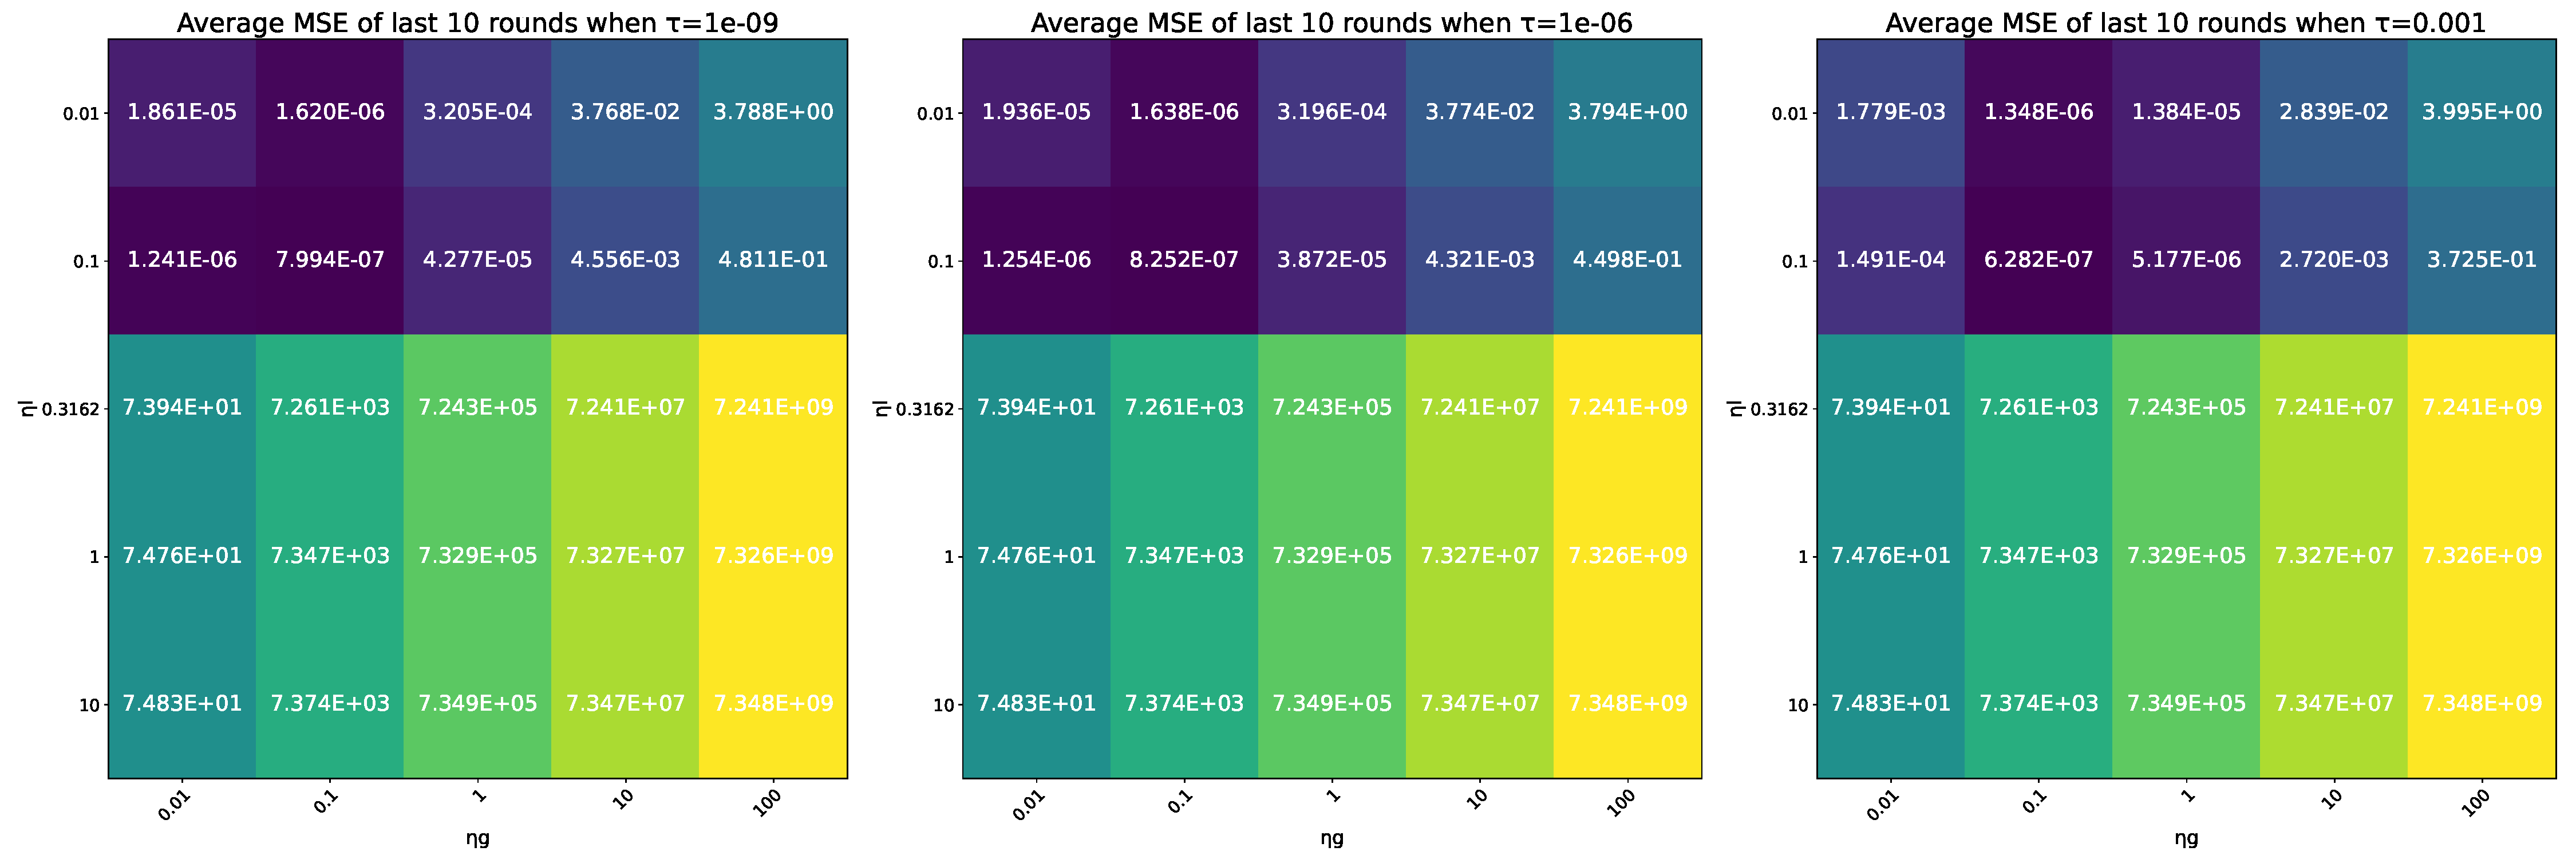
\includegraphics[width=\linewidth]{figs/fedAdamSyntheticHyperpameterTuning.pdf}}
    \caption{Hyper-parameter sweep of FedAdam for the synthetic data set}
    \label{fig:fedAdamSweep}
\end{figure}

Hydra is used to allow easy management of the configuration of the runs of the baseline, and to manage the hyper-parameters -- this makes it very easy to change any of the values, for example the size of mini-batches, number of local epochs, concentration of Dirichlet distribution etc., controlled by YAML config files.  The YAML config files supplied with the baseline will produce the same results as in the original FedExP paper (with the optimal hyper-parameters selected for each strategy with exception of FedAdagrad the reasoning behind this is explained \ref{Analysis}).  The use of configuration files makes it very easy to add in new strategies to the comparison on any data set and perform hyper-parameter tuning; FedAdam has been added as an additional algorithm compared to the original paper for use on the synthetic data set, to add it to the comparison a single new YAML file had to be created specifying where to find the strategy (the FedAdam strategy is already built into Flower so this is referencing that implementation), and the hyper-parameters associated with that strategy (but none of the general hyper-parameters which affect all strategies).  To perform a hyper-parameter sweep Hydra can be used in multi-run mode, where several values for each hyper-parameter can be specified and the baseline is run across all combinations the results of the hyper-parameter sweep for FedAdam on the synthetic data set can be seen in figure \ref{fig:fedAdamSweep} (the values for $\beta_1$ and $\beta_2$ are kept at 0.9 and 0.99 respectively, as was done in \cite{AdaptiveFederatedOptimisation}).

\section{Analysis}
\label{Analysis}

The analysis of FedExP and comparison to other strategies will mainly focus on the synthetic data set because of limited computational resources available to me, which means that it is the only data set where I can run it for a significant number of rounds with similar settings to the paper; and there are interesting observations which can be made on this simple problem.  There is also a brief look at the initial performance of the strategies on other data sets however these runs are not necessarily identical to the original paper (this was again caused by limited computational resources), and potentially do not use optimal hyper-parameters for the new runs so any conclusions which can be made from them are more limited.

It is also the case that SCAFFOLD is not included in the comparison of the different strategies, despite being included in the original paper, because it is natively available inside of Flower and was not inside the scope of this project to implement (although when it becomes available in Flower it will be simple to add), however FedProx has been included despite not being included in the main part of the original paper.  It should also be noted that the implementation of FedAdagrad used differs from the one used in the original paper, in where the adaptability parameter is added (in the Flower strategy it is outside a square root but the original paper has it inside) which cannot be simply corrected by some constant adjustment.  Therefore it is likely that the results for FedAdagrad could be improved by redoing hyper-parameter tuning, this would not affect the synthetic data set anyway (because it is set to 0) and I have not had the computational resources/time to be able to perform it for the other data sets where it would likely make a difference.

\subsection{Synthetic data set}

\subsubsection{Comparison of different seeds for data set generation}

The performance of the different strategies is shown in figure \ref{fig:200RoundsSeed0} when run on exactly the same synthetic data set as in the original paper.  From the graph it is clear that the performance of FedExP is the same as is shown in the original paper.  The more spiky nature of all of the lines of the plots (and fast oscillations in FedAdagrad) are caused by taking the evaluation of the model after every round instead of every five rounds.  It is clear that FedExP is converging towards the optimal solution substantially faster than any of the other methods, including FedAdam which was not included in the original paper.  It is also clear from these graphs that having a very high global learning rate is important for solving this problem quickly because FedProx (which is a very strict implementation where the global learning rate must be one) is performing significantly worse than the other methods.  This observation may not be particularly helpful with real problems because they are generally so complex that a really high global learning rates will not be helpful (leading to problems with no/slow overall convergence).  However it does show that if for a real task a very high global learning rate can be used effectively (even if just temporarily) then FedExP should be able to best exploit it by dynamically changing the learning rate.  Figure \ref{fig:200RoundsSeed42} shows that these conclusions are still valid when run on data sets generated with different seeds; it is interesting to observe that FedExP has significantly higher variance on lots of rounds, but also much greater variance in variance, this is caused by the very oscillatory nature of its learning process.

\begin{figure}
    \centerline{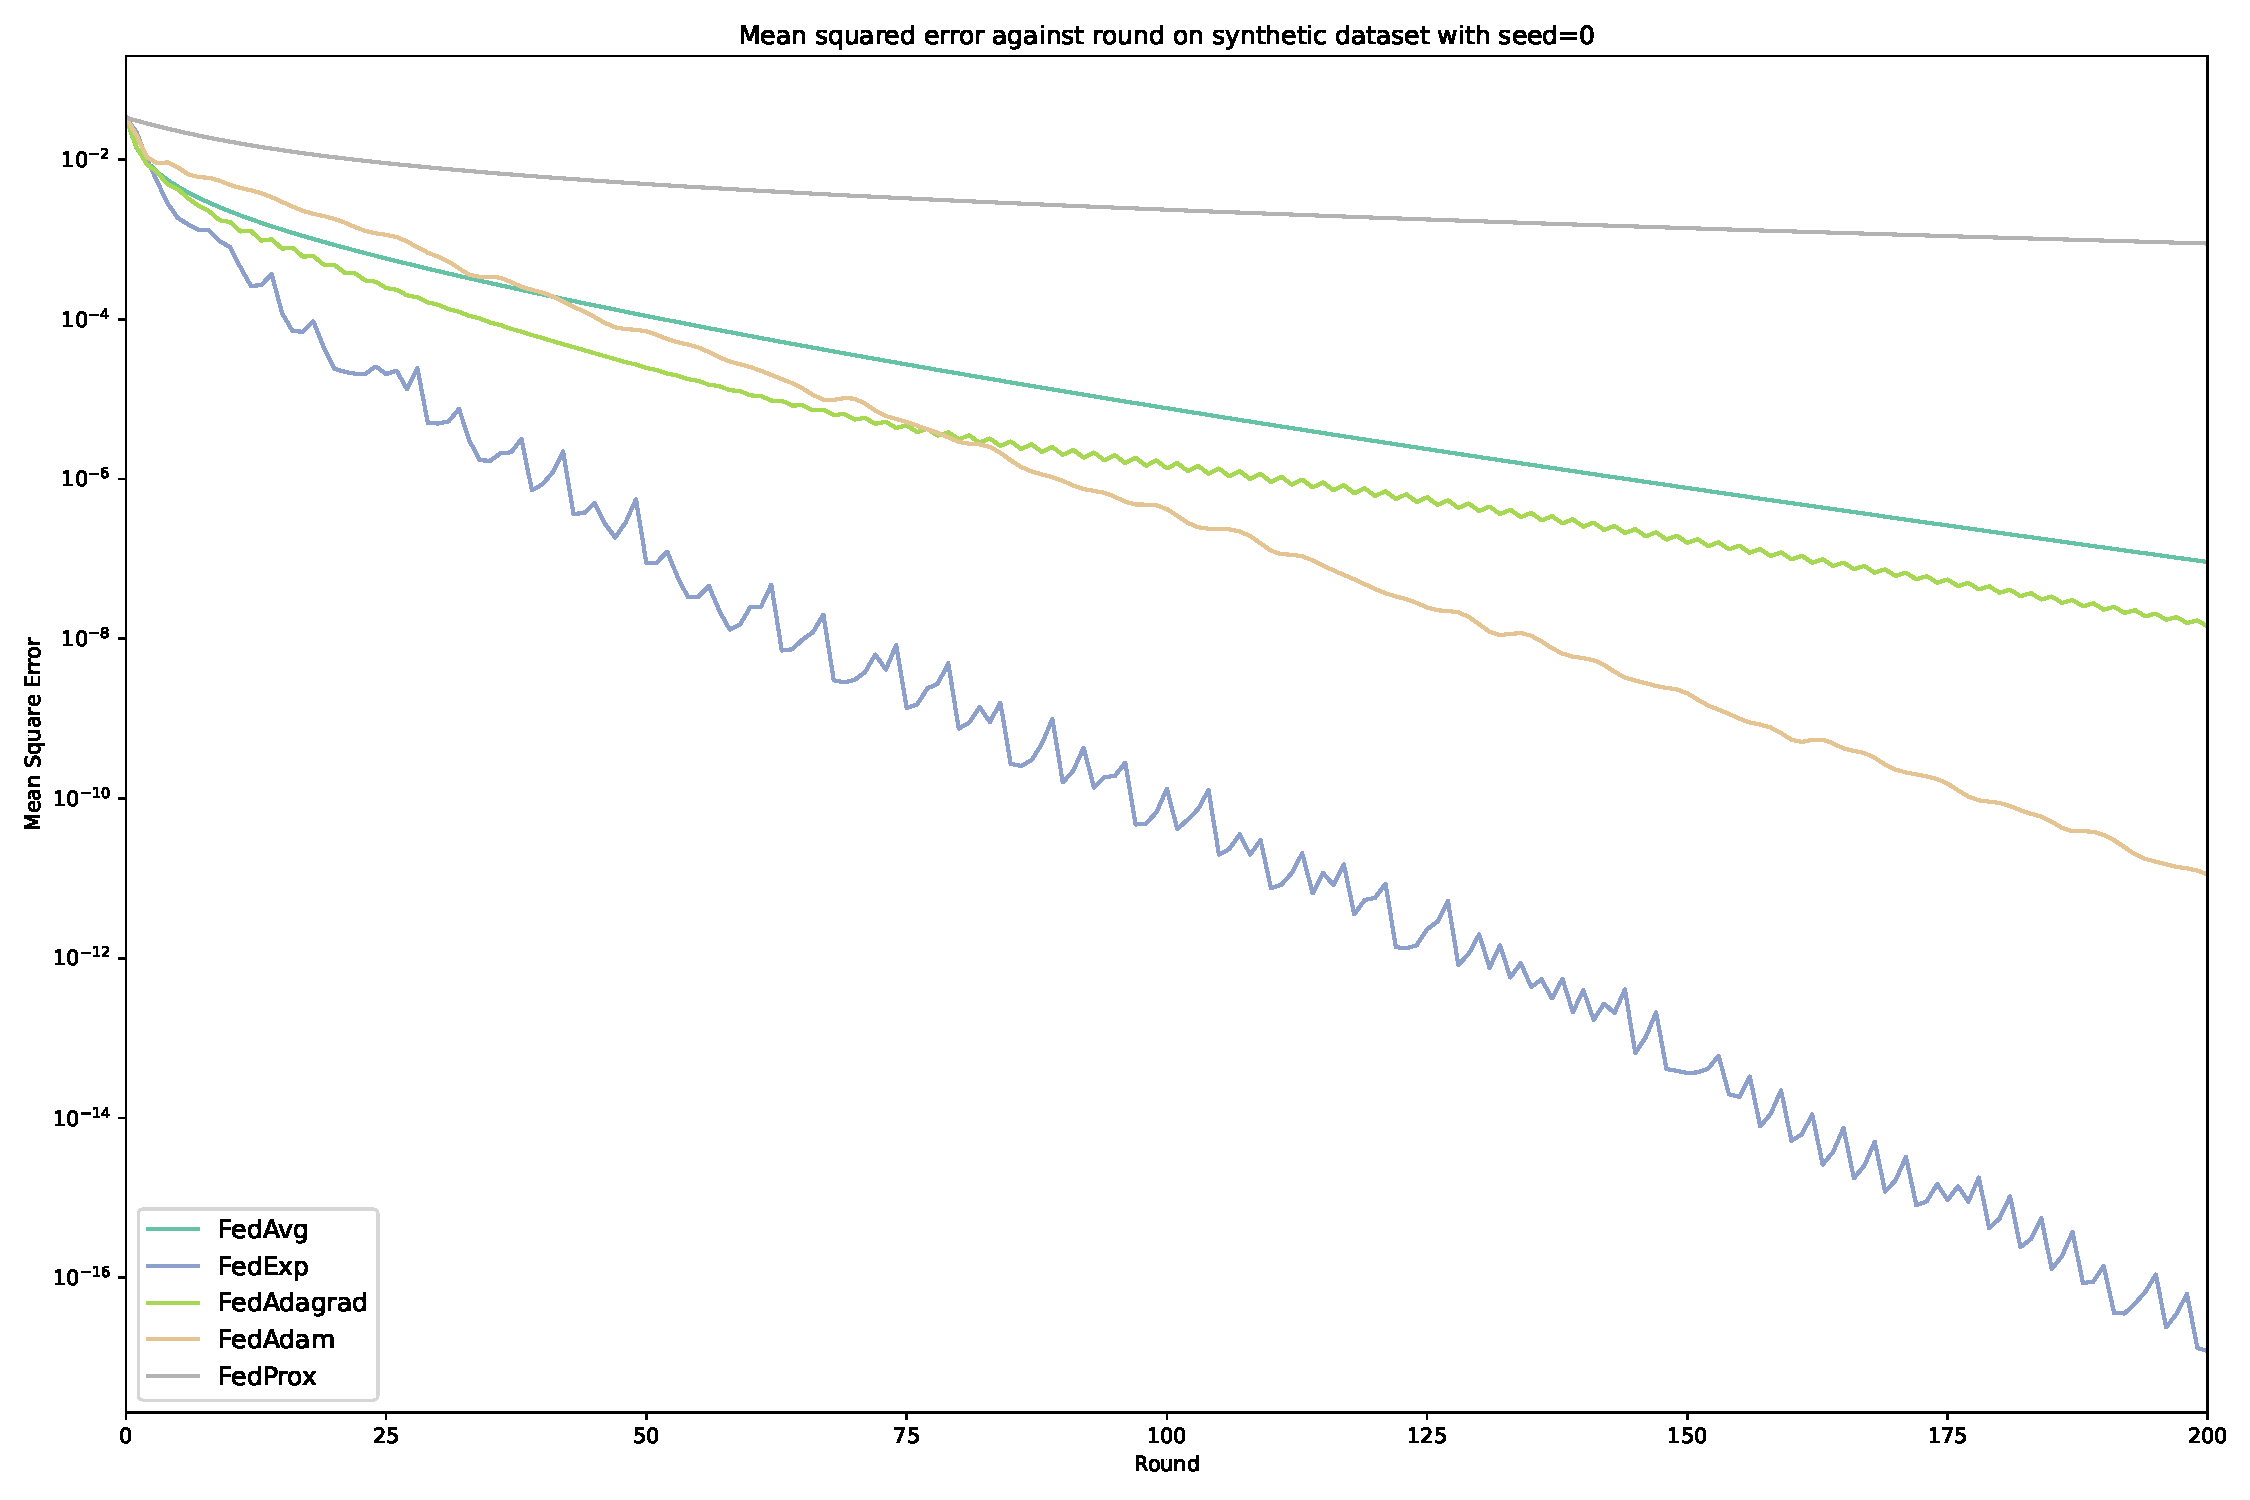
\includegraphics[width=.6\linewidth]{figs/syntheticSeed0_200Rounds.pdf}}
    \caption{Performance of different strategies on the synthetic data set, generated with np.random.seed(0)}
    \label{fig:200RoundsSeed0}
\end{figure}

\begin{figure}
    \centerline{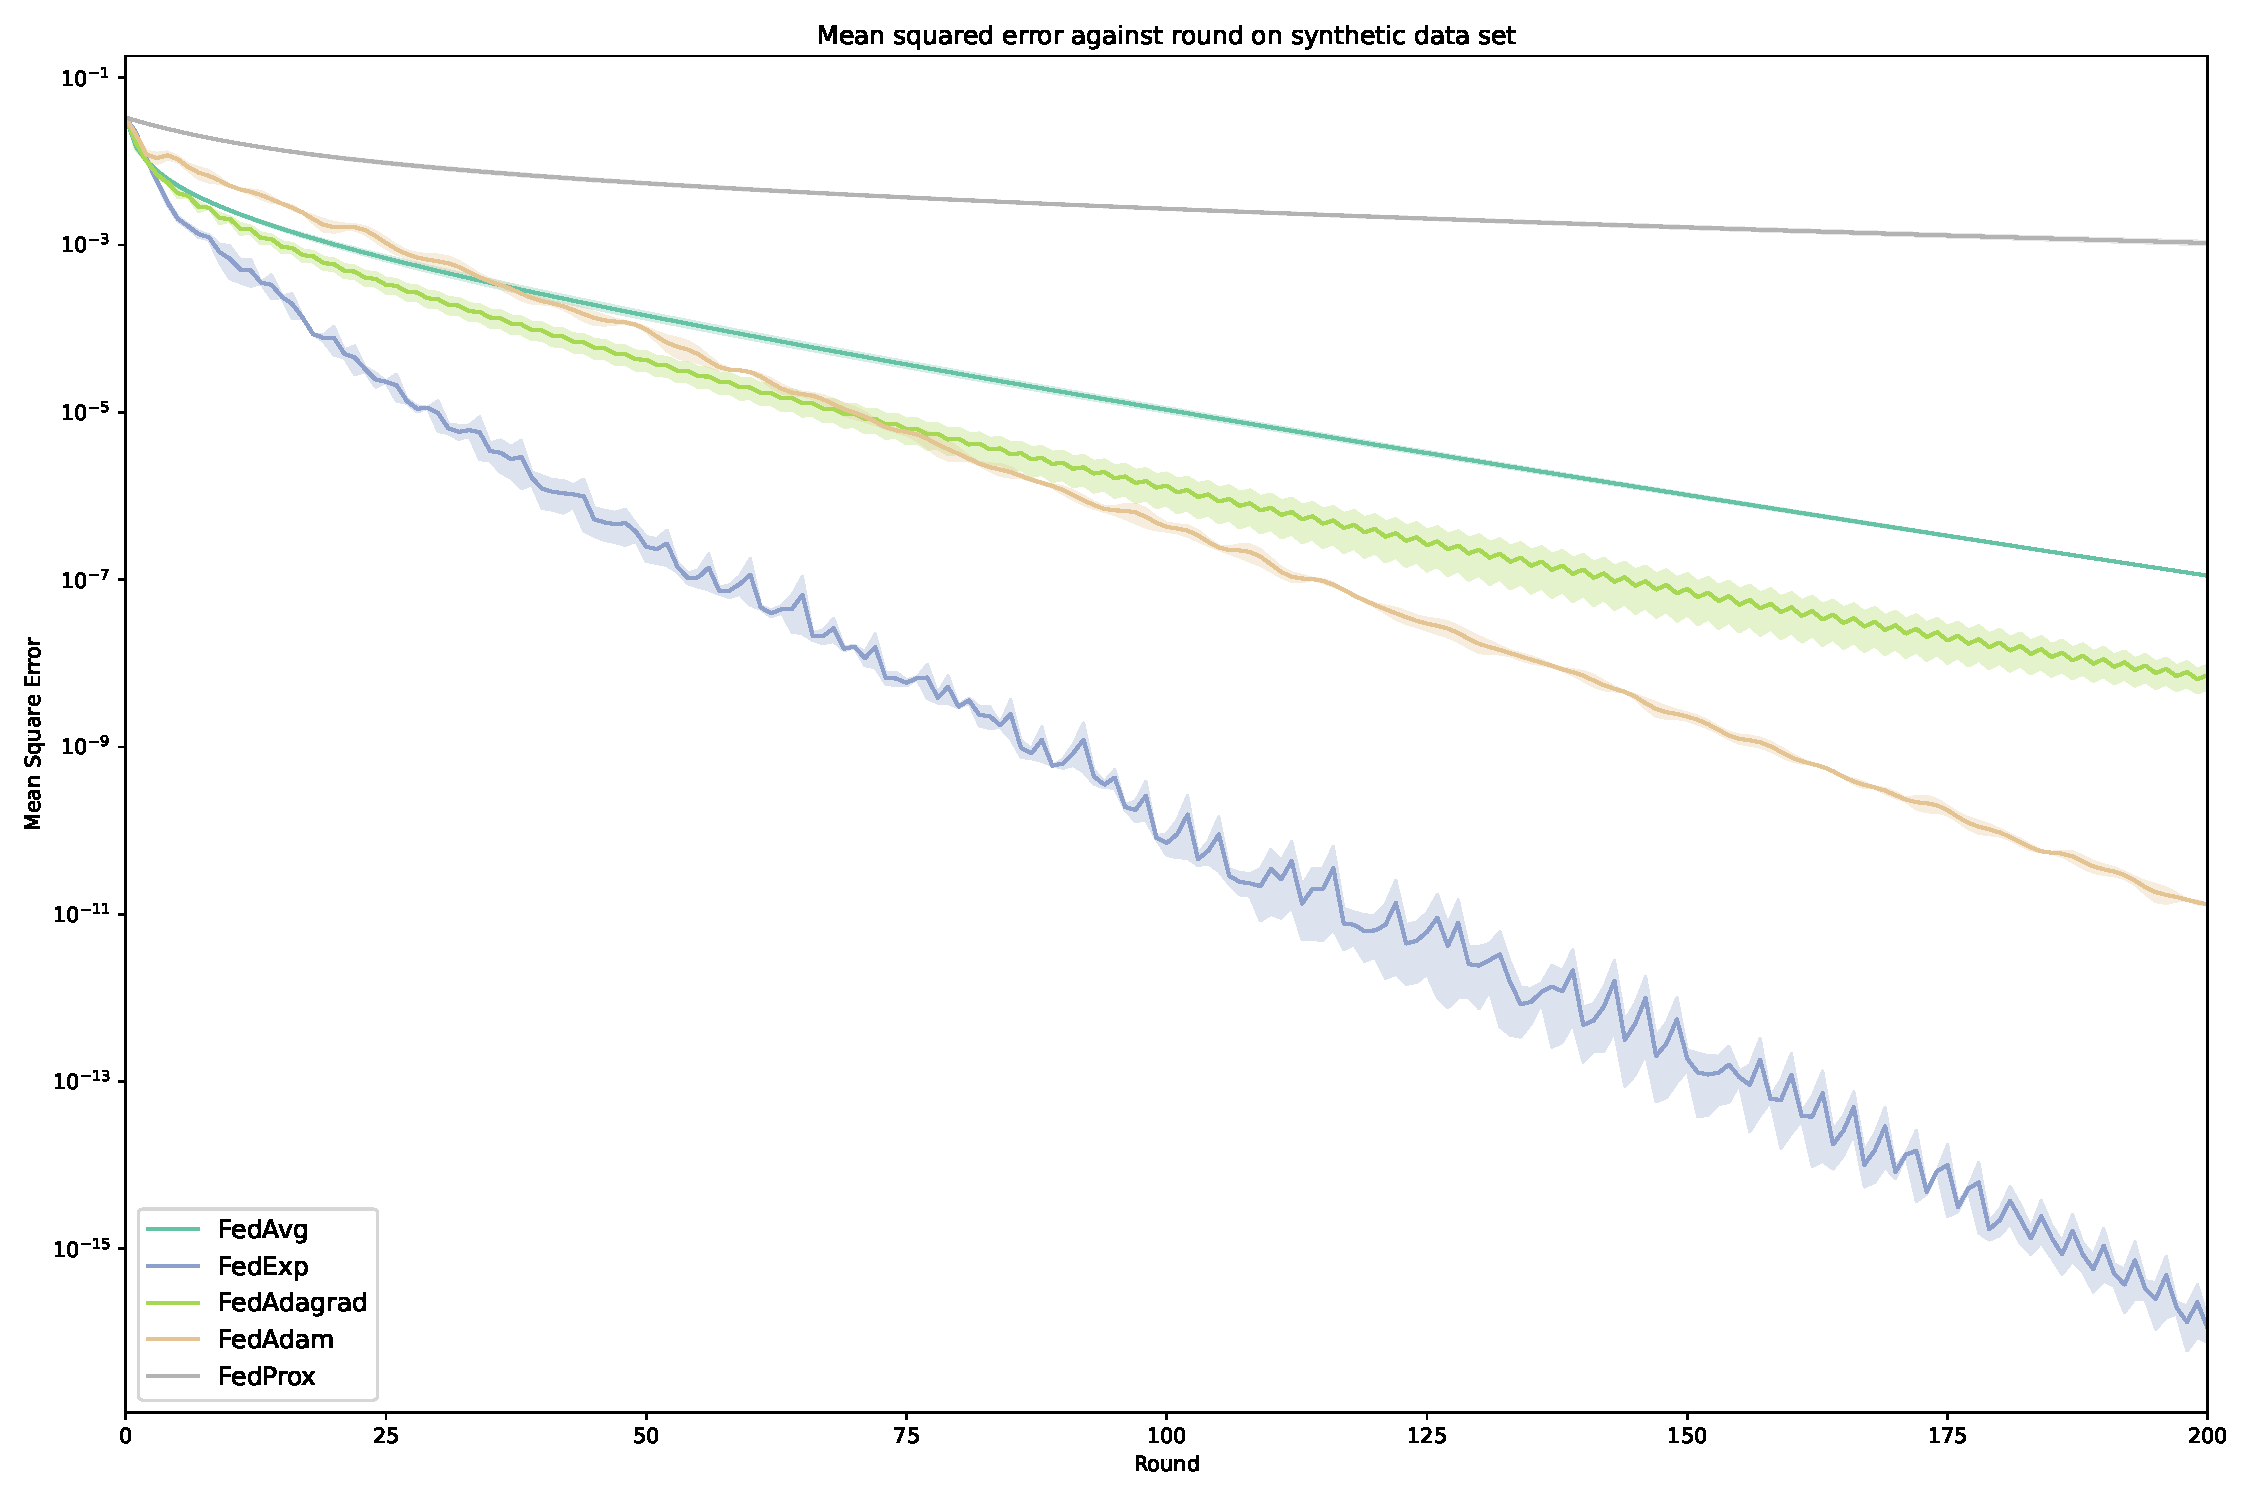
\includegraphics[width=.6\linewidth]{figs/synthetic_200Rounds_ManySeeds.pdf}}
    \caption{Performance of different strategies on the synthetic data set with several seeds used to generate the data set}
    \label{fig:200RoundsSeed42}
\end{figure}


\subsubsection{Effect on evaluation performance of varying the number of rounds averaged over}

Figure \ref{fig:differentNumberOfAverageEvaluateRoundsSynthetic} shows the affect of changing the number of rounds which are averaged out to give the parameters for the evaluation.  As expected the larger the number of rounds averaged over the smoother the loss curve is.  The higher number of evaluation rounds all start their curves with very similar smooth curves, this is caused by the fact that the number of rounds is being increased on every extra round due to not actually having gone through all the rounds which is wanted to be averaged over.  This graph shows a clear trade off between having a much smoother curve and still having low loss, in the original paper they mention how increasing the number of rounds averaged over past 2 did not have much effect but in the synthetic data set it clearly does have a large effect, arguably 5 rounds looks to be the best trade off for this data set.  However in real data sets it is likely that their observations do hold and this higher number is caused by the very easy nature of the problem (leading to very high global learning rates selected) which is being solved. 

\begin{figure}
    \centerline{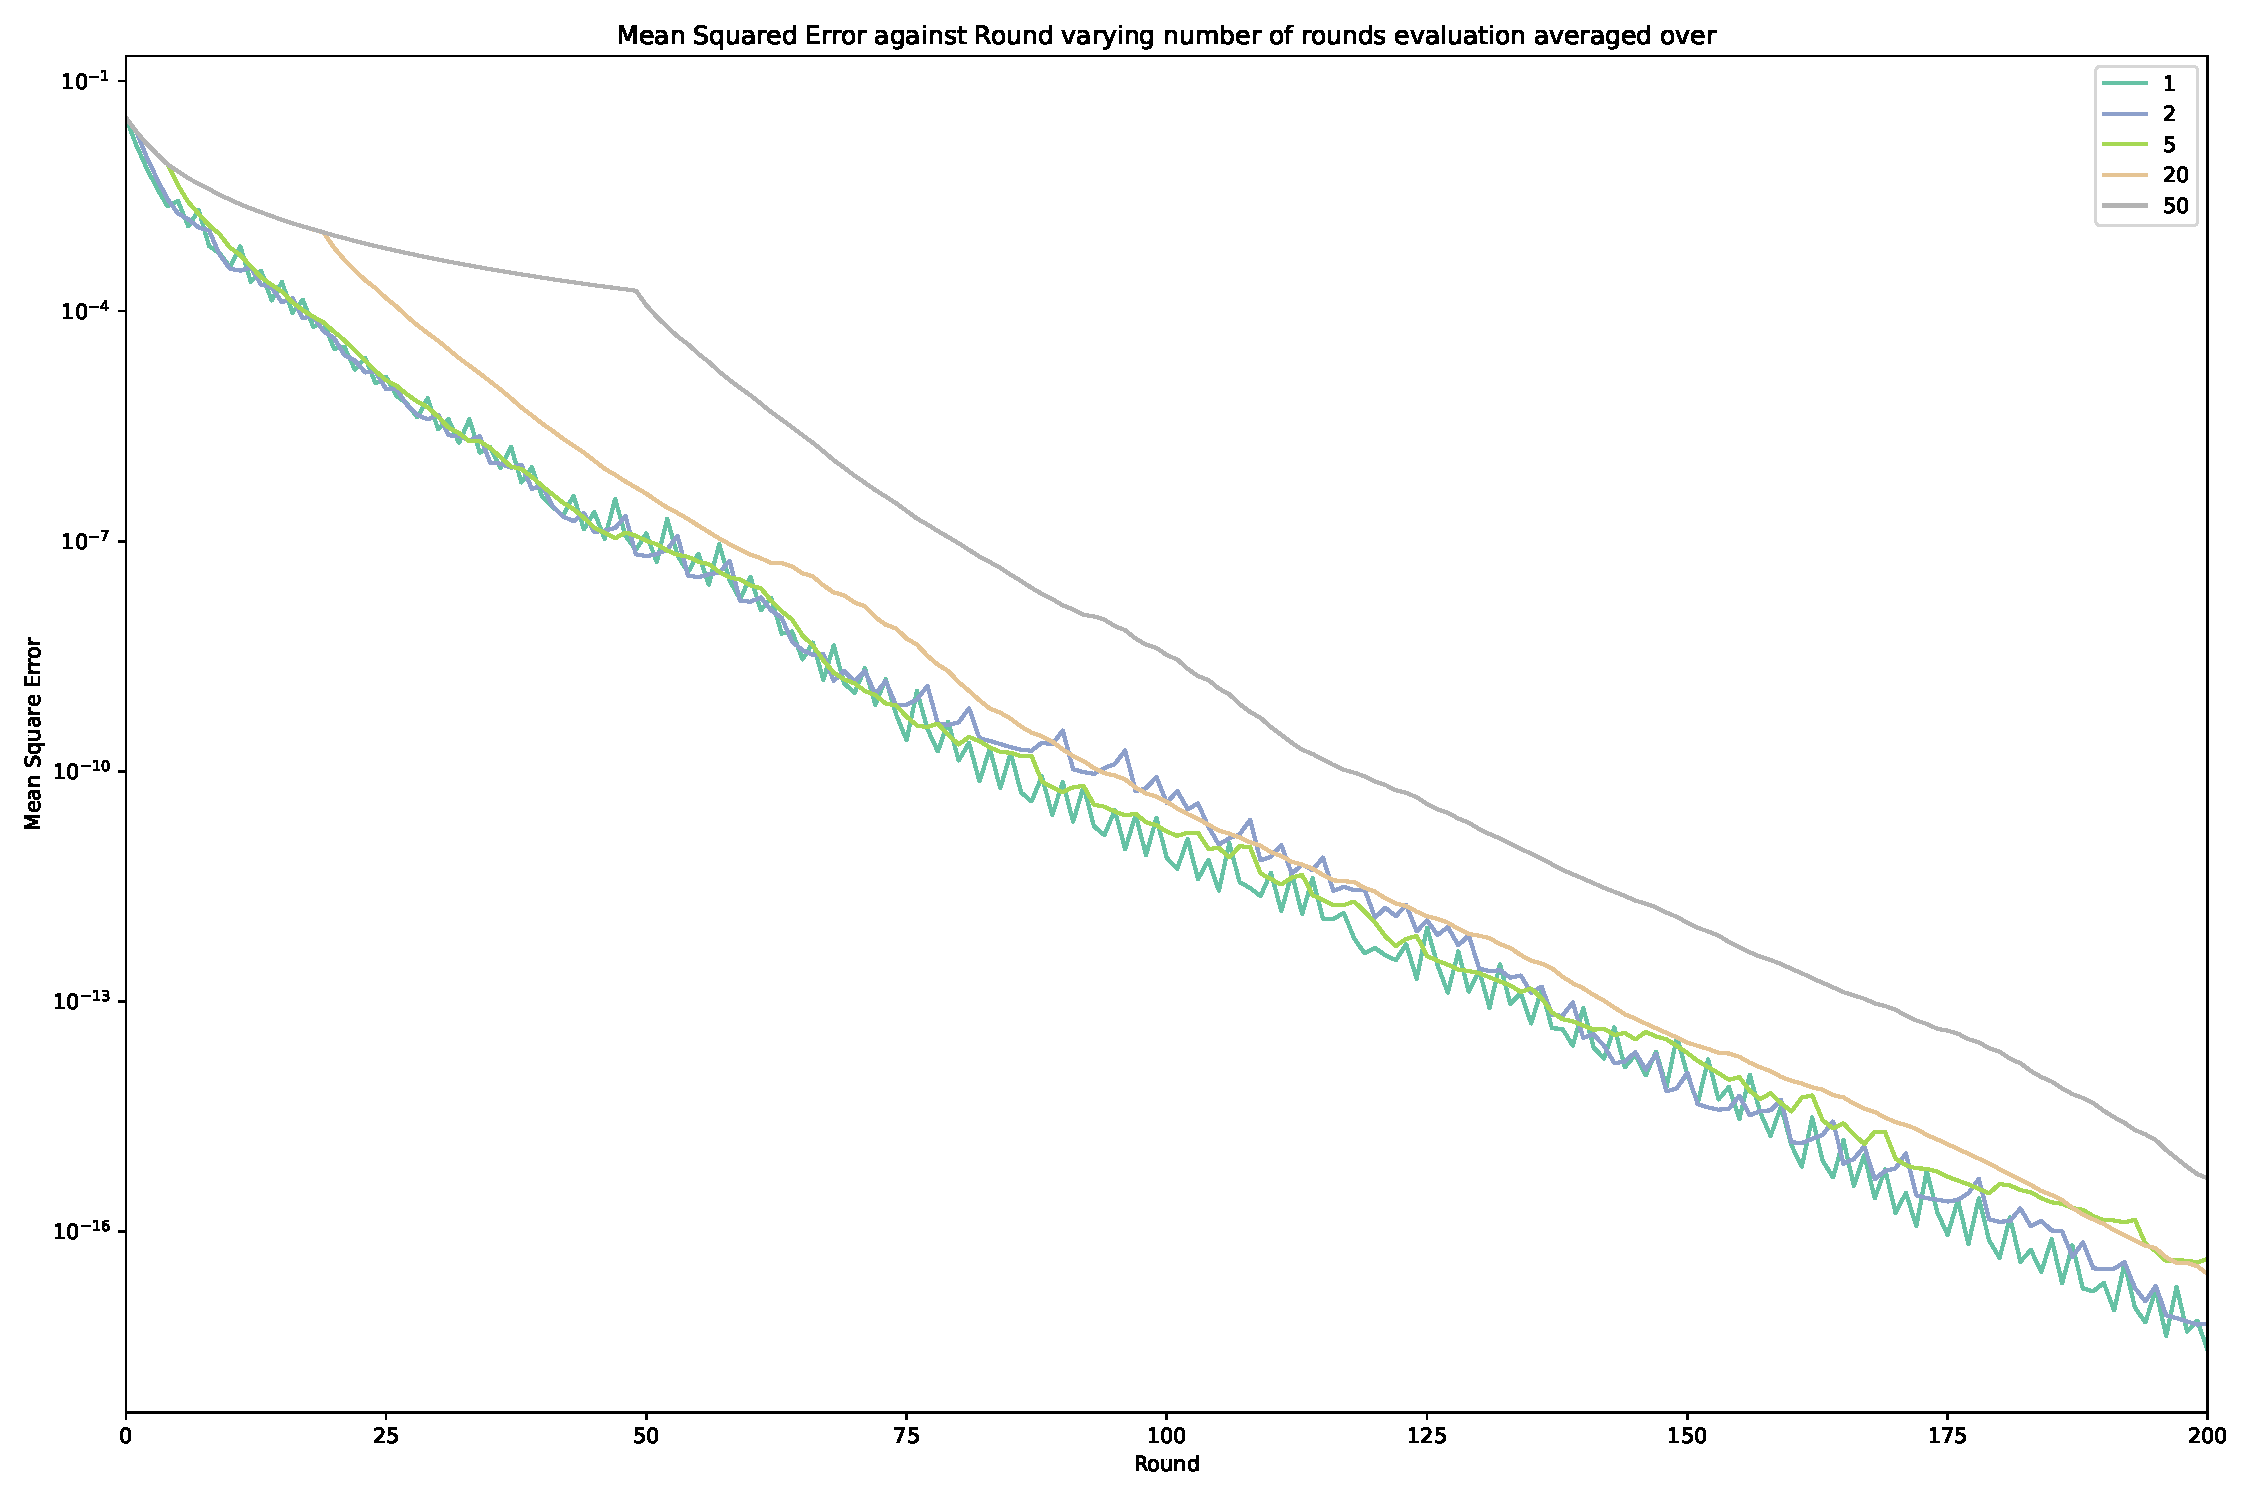
\includegraphics[width=.6\linewidth]{figs/synthetic_numberOfRoundsAverageEvaluate.pdf}}
    \caption{FedExP performance reported in evaluate averaging over different number of rounds}
    \label{fig:differentNumberOfAverageEvaluateRoundsSynthetic}
\end{figure}

\subsubsection{Long term behaviour}

In figure \ref{fig:2000RoundsSynthetic} the performance of the different strategies can be seen over a much larger number of rounds until the point that most of them are not improving any more.  FedProx is clearly the outlier, as before this is due to it having a much smaller global learning rate.  The performance of FedExP is quite interesting to observe because it clearly has the most perturbed loss curve when learning is actually happening but when it has learned the solution it has one of the smoothest curves; this makes sense because during the learning process it will have a very high global learning rate to make big changes but is able to lower the global learning rate dynamically to ensure that the weights are still getting closer to the optimal set of weights and can turn into FedAvg when the value suggested by extrapolation is small.  It is also clear from the graph that the end of performance of FedExP is actually higher than any other methods (although if run for a few thousand more rounds then it is likely that FedAvg would get very close), this shows that for this problem it is clearly the best strategy and has the good theoretical results in practice and that compared to other adaptive strategies it is not suffering from achieving a lower end performance compared with more simple strategies.

\begin{figure}
    \centerline{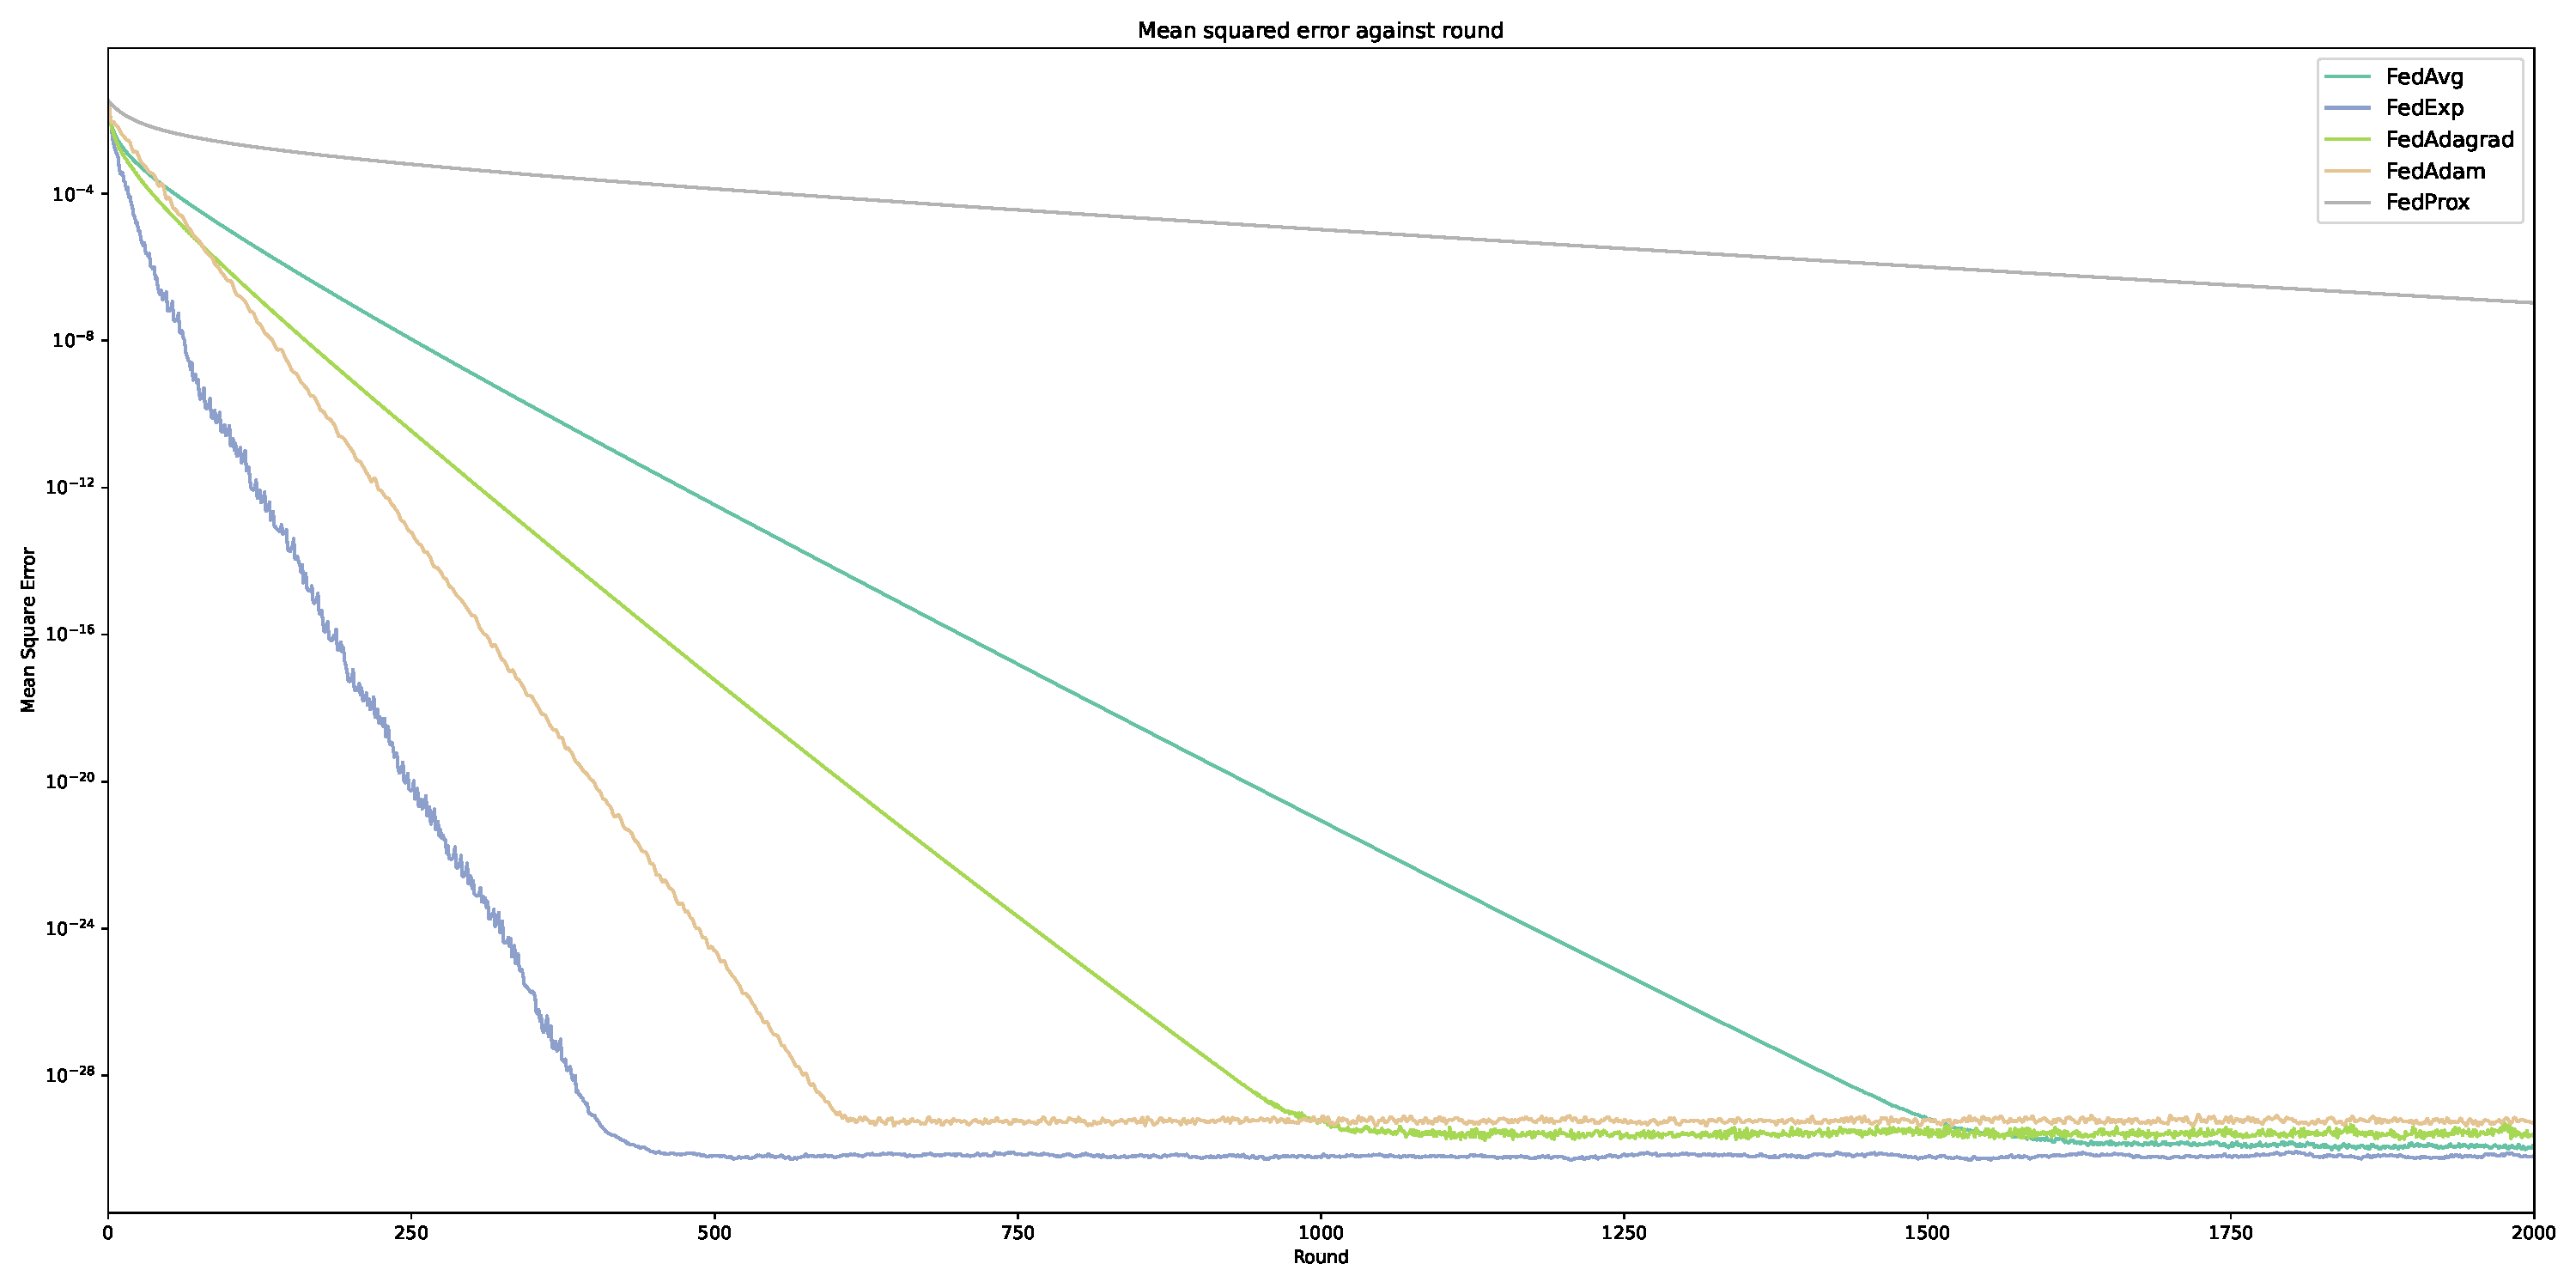
\includegraphics[width=.85\linewidth]{figs/synthetic_2000Rounds.pdf}}
    \caption{Performance of different strategies on the synthetic data set}
    \label{fig:2000RoundsSynthetic}
\end{figure}

\subsubsection{Varying $\epsilon$}

\begin{figure}
    \centerline{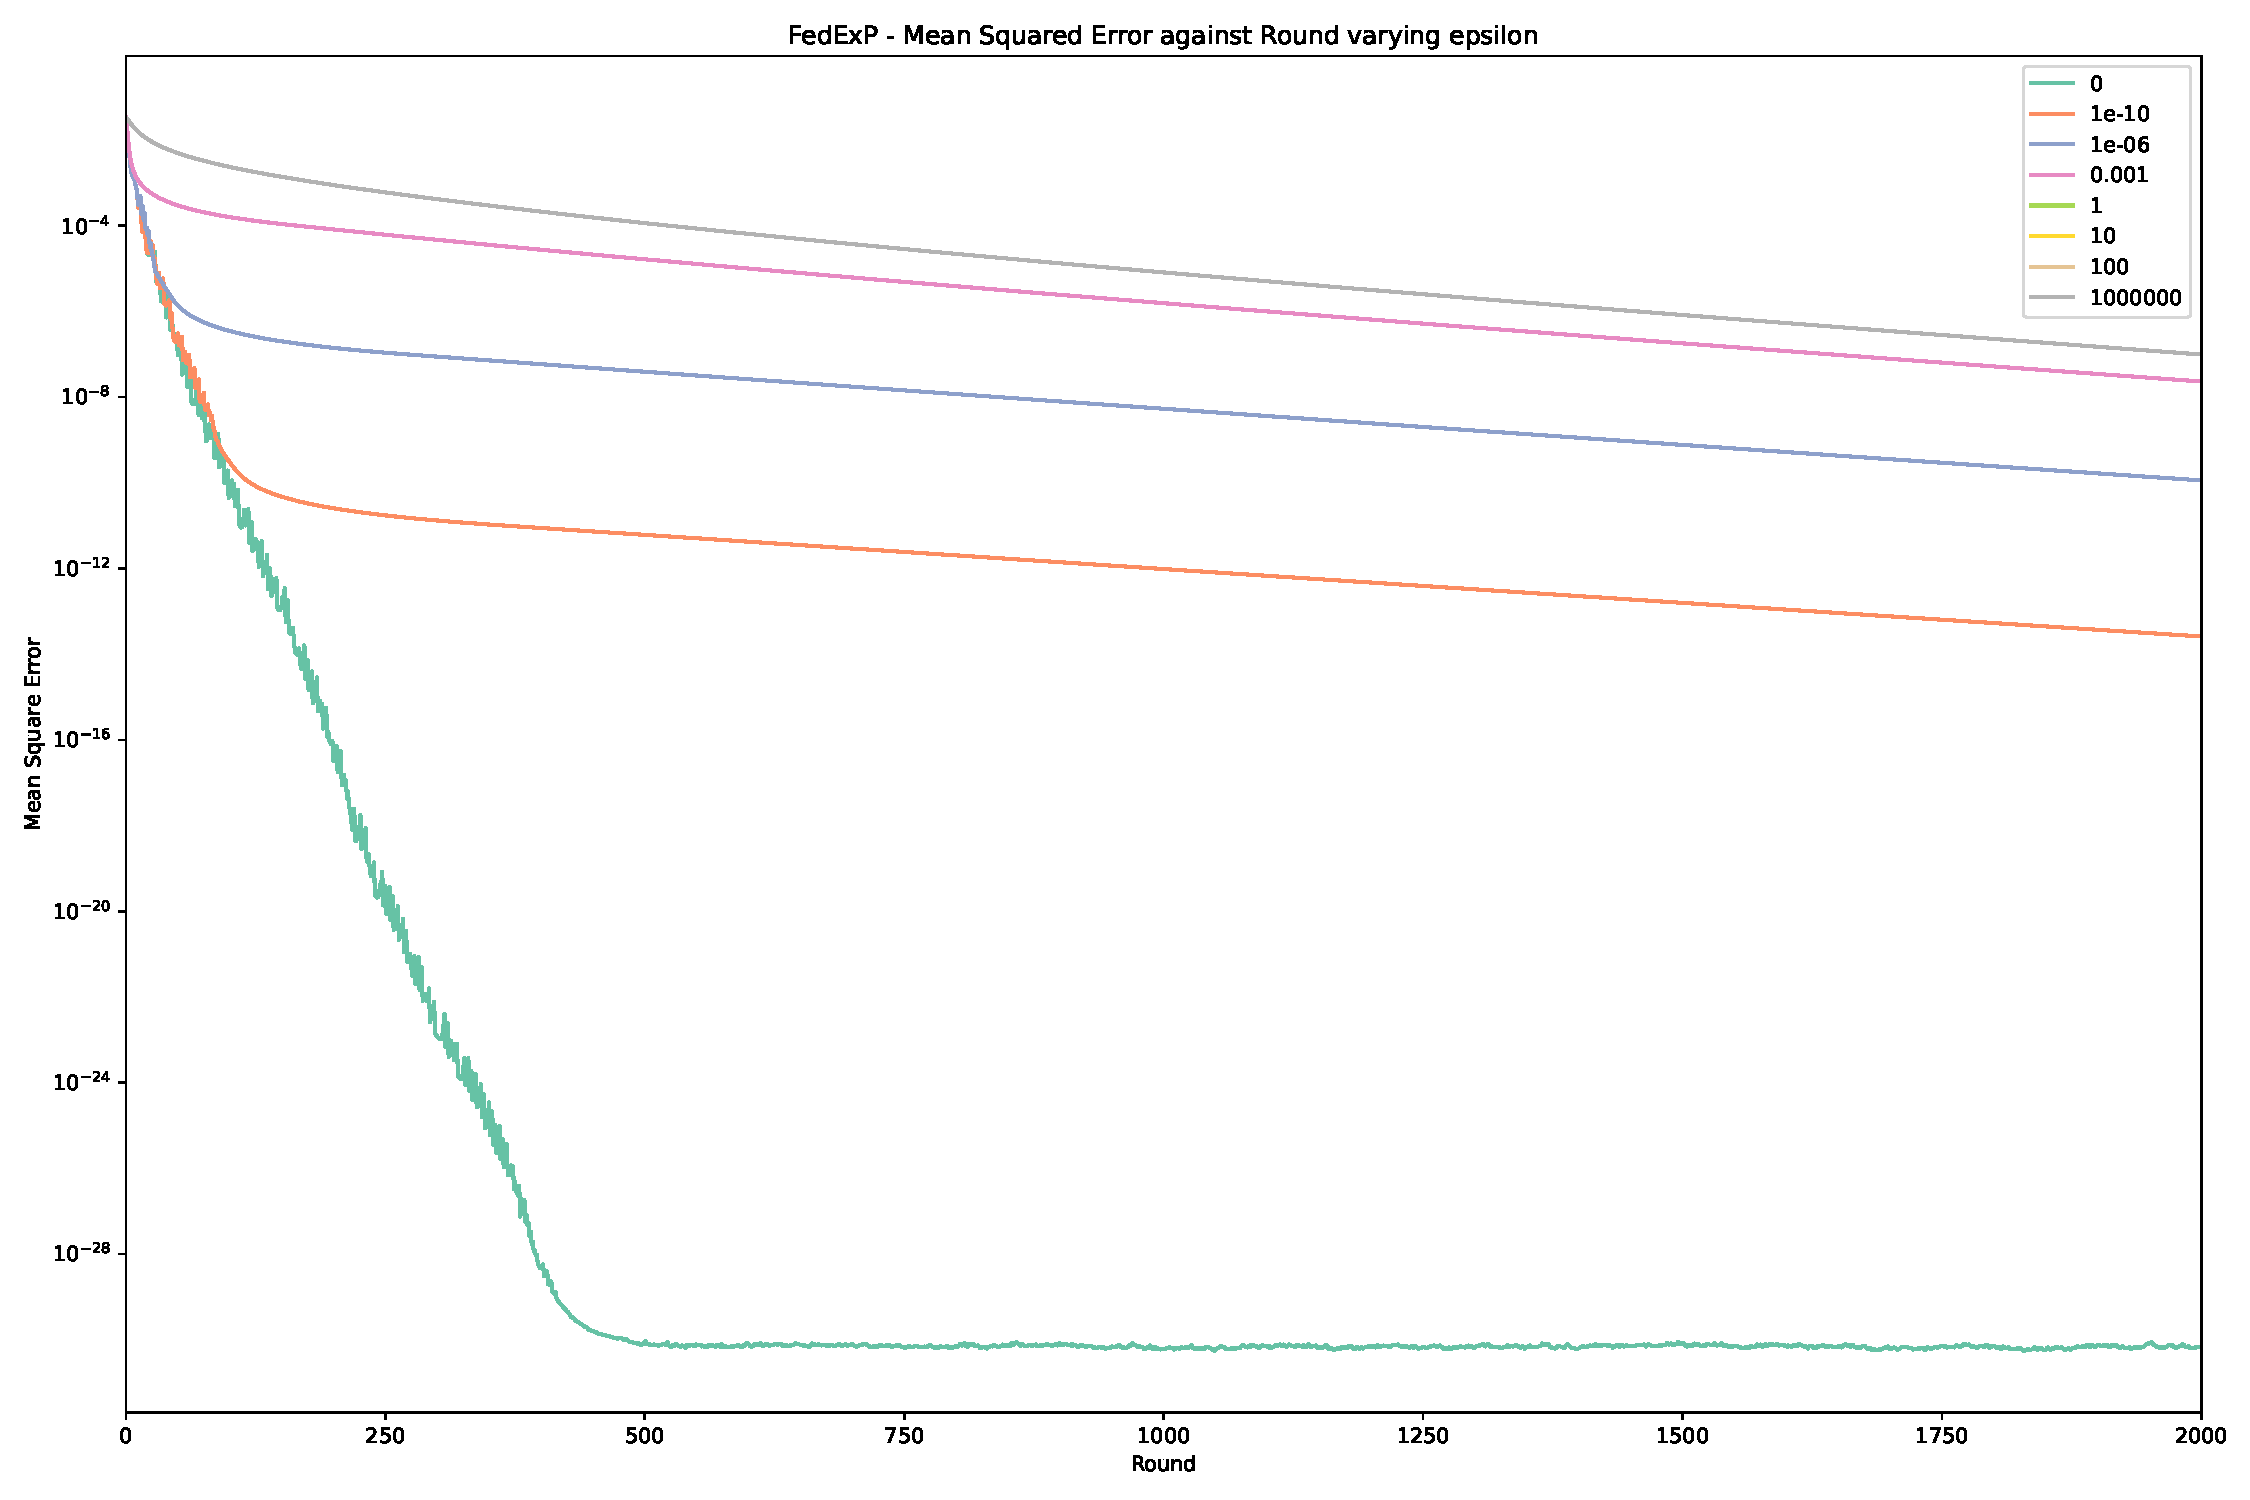
\includegraphics[width=.85\linewidth]{figs/synthetic_varyingEpsilon.pdf}}
    \caption{Performance of FedExP with varying $\epsilon$}
    \label{fig:varyingEpsilon}
\end{figure}

In figure \ref{fig:varyingEpsilon} the effects of changing the value of $\epsilon$ can be seen.  It is clear that having a higher value for $\epsilon$ leads to a smoother curve (because it is going to be using a smaller global learning rate therefore changes will not be as extreme to the overall model), while leading to significantly slower convergence to the optimal model.  The extreme sensitivity of performance to $\epsilon$ is likely to be a slight quirk of this data set, because the global learning rate chosen if not following the extrapolation is 1 but for the other strategies where the global learning rate is tuned it is set to 10, however the main point still stands in that increasing $\epsilon$ leads to performance closer to what FedAvg would achieve, it is also the case that above a certain point changing it has no effect because the extrapolation will never be chosen as the value for global learning rate.  The exact values of $\epsilon$ which should be chosen will depend on the model, due to that changing the size of the pseudo-gradient which is expected on each round, and the desired behaviour, if a smoother learning curve is desired then a higher value will likely help but could slow down learning.  It is also possible that an adaptive method for choosing $\epsilon$ could provide advantages, because as explained in the original paper it is mainly useful for when near convergence to the optimal solution, preventing massive learning rates caused by dividing by a value close to zero, therefore increasing $\epsilon$ in later rounds could allow a good blending between the fast learning of FedExP and smooth performance of FedAvg when near optimal solutions.

\subsection{Real data sets}

\begin{figure}
    \centerline{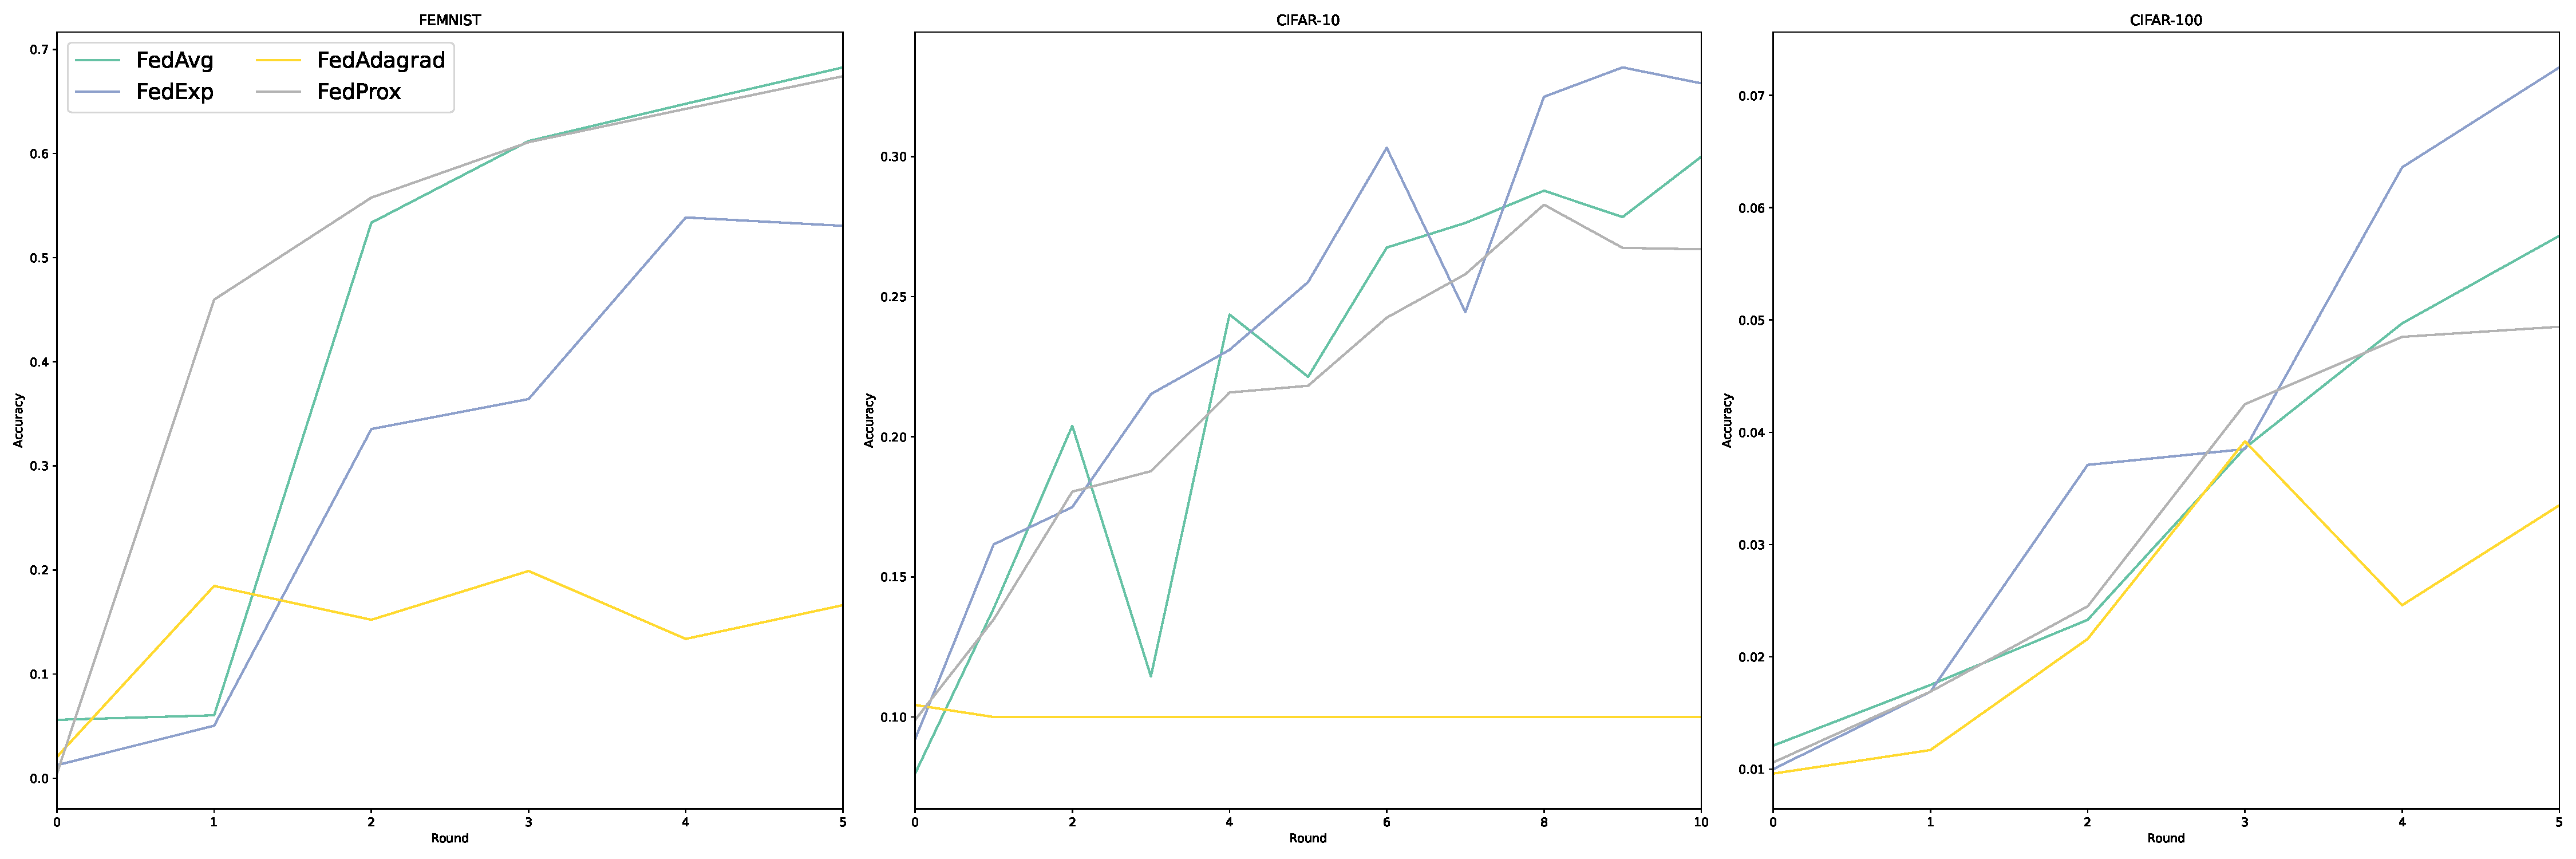
\includegraphics[width=\linewidth]{figs/realDatasetPerformance.pdf}}
    \caption{Performance of different strategies against real data sets}
    \label{fig:realDatasetPerformance}
\end{figure}

In figure \ref{fig:realDatasetPerformance} the performance of the different strategies, for the first few rounds, is shown on several real data sets, it can be seen that FedExP is generally performing well in comparison to the other strategies (for FEMNIST this does not look to hold but would likely be born out in longer runs, because it is making the most progress at the end of the plot); this is supported by what is shown in the paper where it is expected that FedExP will achieve faster convergence by dynamically selecting a good global learning rate.  The slight caveats to this are that FedAdagrad is not performing very well at all, this is likely due to mischosen hyper-parameters because of the differences between the FedAdagrad implementations explained above, and the settings used for the CIFAR data sets differ to those in paper due to limited computational resources (only using 3 local epochs and 10 clients per round).  However this still shows that dynamically altering the learning rate can lead to better performance.

\subsubsection{FEMNIST evaluate number of rounds}

In figure \ref{fig:femnistDifferentNumberOfEvaluateRounds} it is clear that the performance of FedExP is increased by averaging the weights used in evaluation compared to the raw weights, because a lower global loss region is being followed, and that it has smaller perturbations in the loss curve getting closer to the performance of FedAvg (and would likely surpass if trained for more rounds).  This clearly shows that when working on real data sets it is important to average out several rounds of weights when evaluating the performance of the model, potentially more so than on the synthetic results because of the noticeably higher performance in this more difficult task.

\begin{figure}
    \centerline{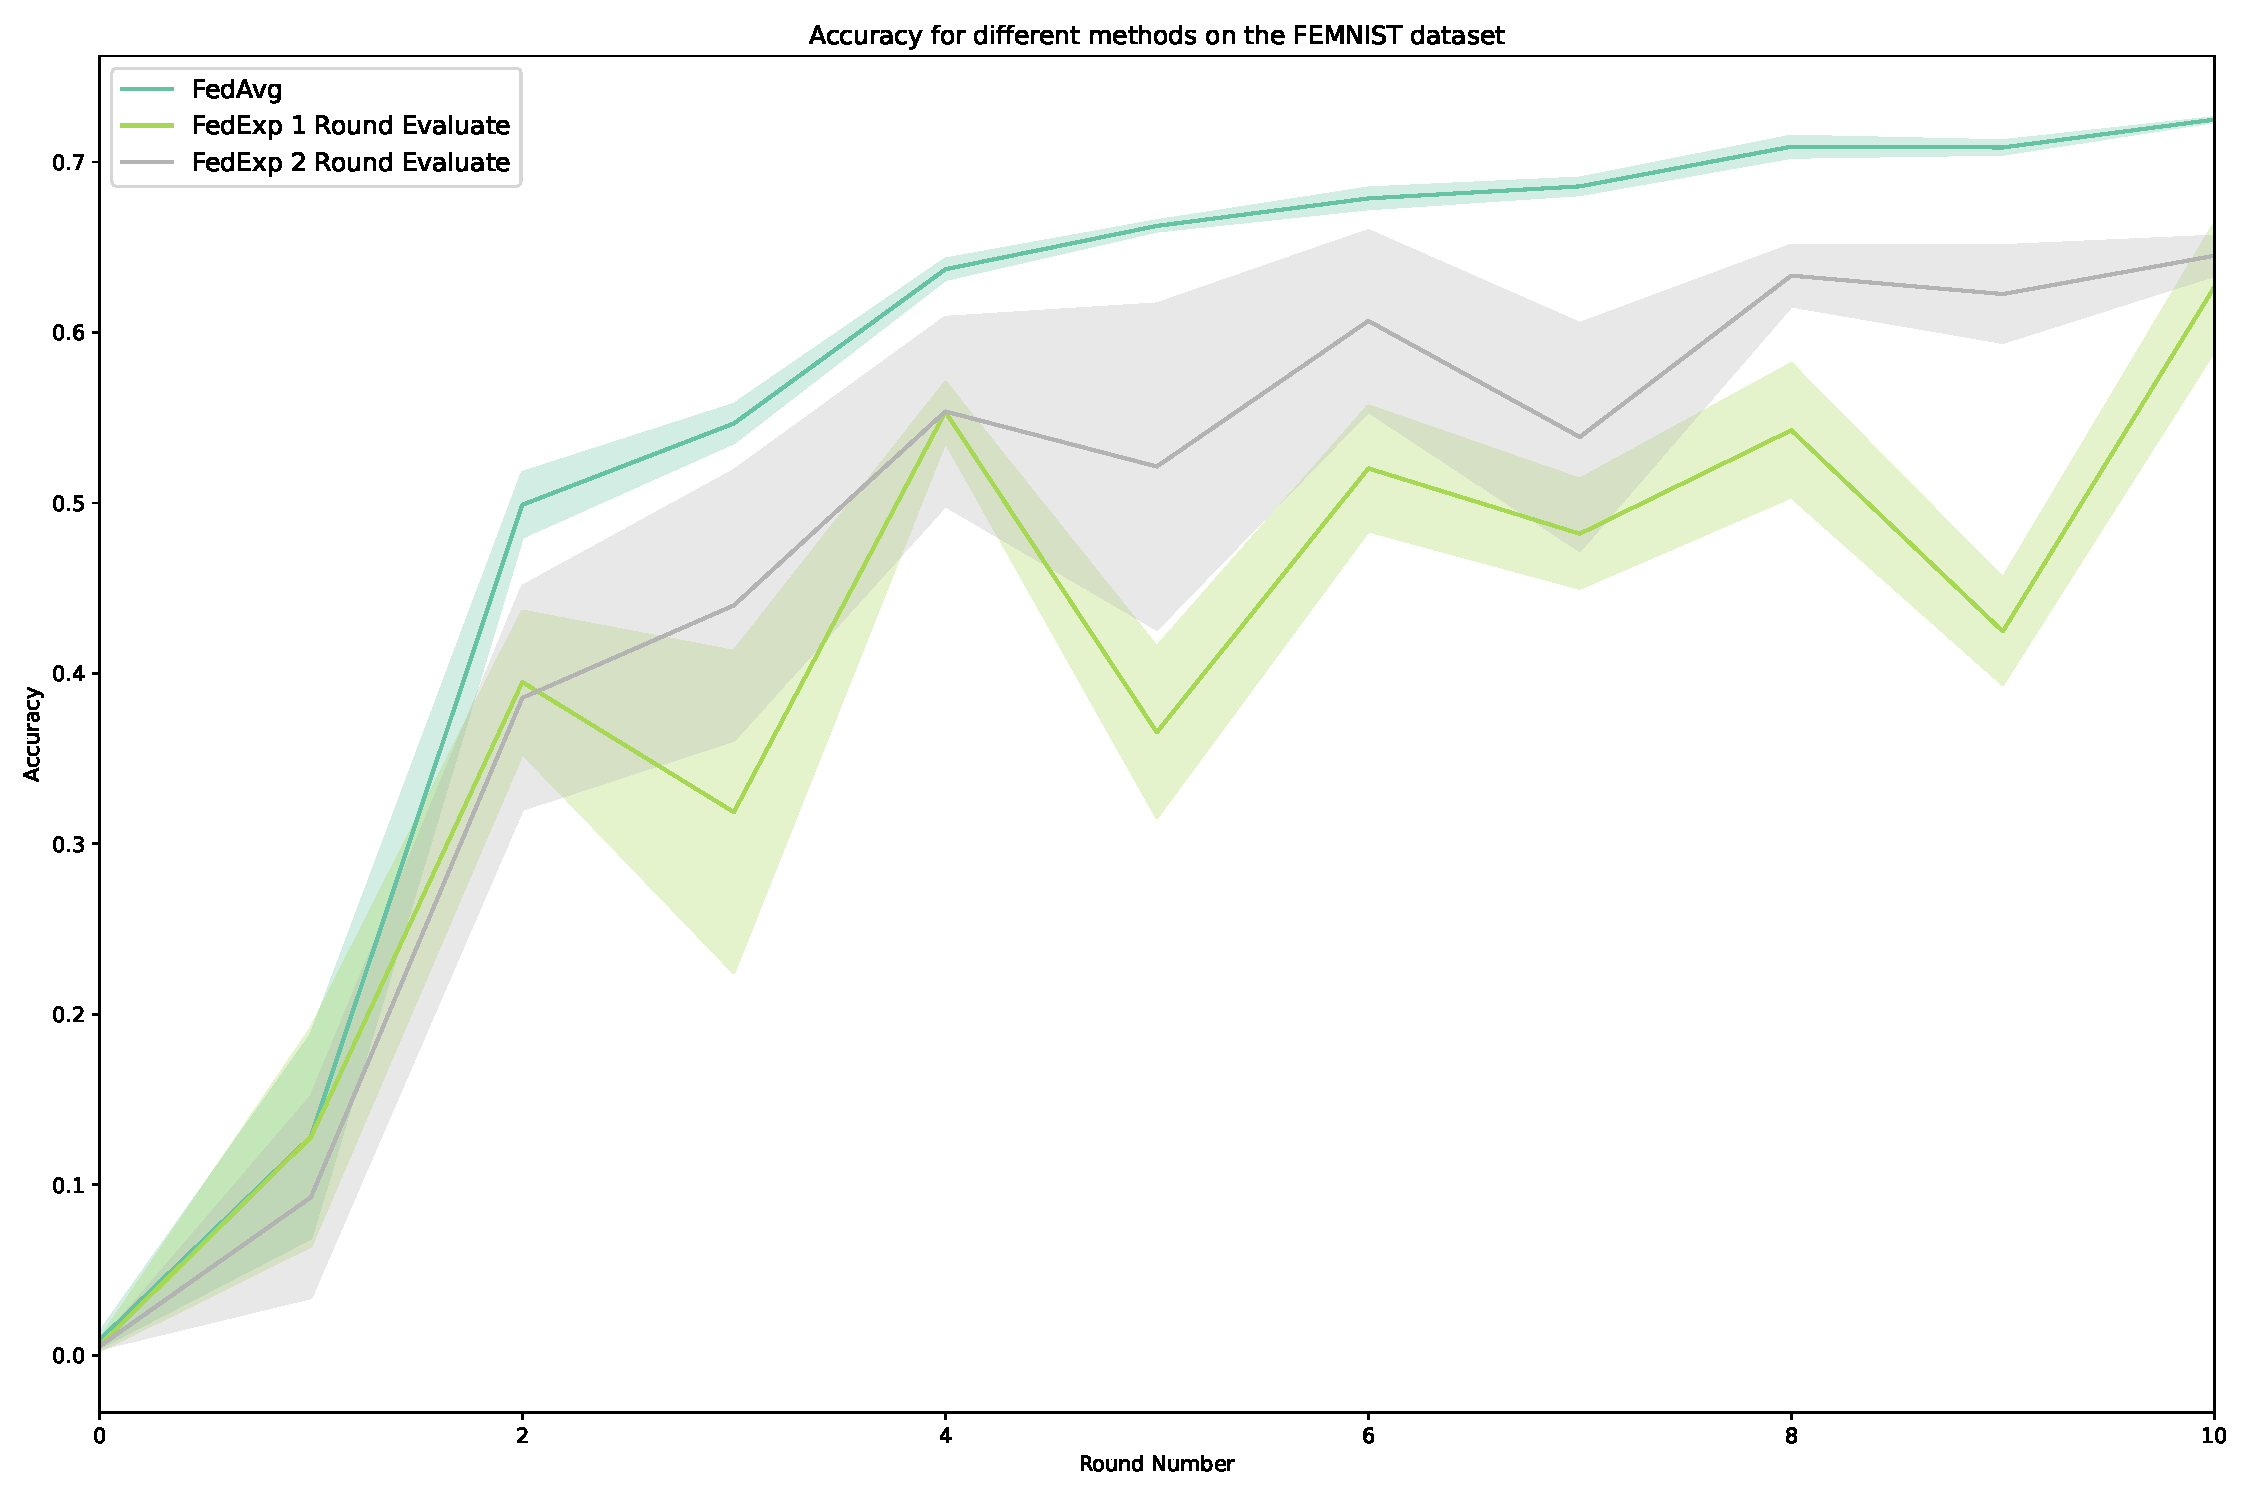
\includegraphics[width=.6\linewidth]{figs/femnist_fedexp_fedavg_evaluateRounds.pdf}}
    \caption{Performance of differing number of average rounds for FedExP against FedAvg on FEMNIST data set}
    \label{fig:femnistDifferentNumberOfEvaluateRounds}
\end{figure}

\section{Conclusion}

This project has successfully implemented the FedExP strategy into Flower and provided an analysis and comparison of its performance, with attention paid to how varying its hyper-parameters' change its behaviour.

\bibliography{refs}

\end{document}
